% vim: set spell spelllang=en tw=100 et sw=4 sts=4 :

\documentclass[a0paper]{tikzposter}

\usepackage{complexity}
\usepackage{wrapfig}
\usepackage{microtype}
\usepackage{gnuplot-lua-tikz}
\usepackage{amssymb}
\usepackage{amsmath}
\usepackage{sfmath}

\usepackage{lmodern}
\renewcommand*\familydefault{\sfdefault}
\usepackage[T1]{fontenc}

\title{Between Subgraph Isomorphism and Maximum Common Subgraph}
\author{Ruth Hoffmann, Ciaran McCreesh and Craig Reilly}
\institute{University of Glasgow, Glasgow, Scotland}
\titlegraphic{\includegraphics[keepaspectratio=true,scale=3.5]{UoG_keyline.pdf}}

\settitle{
    \begin{tikzpicture}
        \node (T) [inner sep=0pt] {\begin{minipage}{\linewidth}
                \color{titlefgcolor}
                {\bfseries \Huge \hspace*{10mm}Between Subgraph Isomorphism and \\
                \hspace*{10mm}Maximum Common Subgraph \par}
                \vspace*{1em}
                {\Large {\bfseries \hspace{10mm}\@author}, \@institute}
        \end{minipage}};

        \node at (T.east) [anchor=center, inner sep=0pt, xshift=-12cm] {\@titlegraphic};
    \end{tikzpicture}
}

% University of Glasgow standard colours
\definecolor{uofguniversityblue}{rgb}{0, 0.219608, 0.396078}

\definecolor{uofgheather}{rgb}{0.356863, 0.32549, 0.490196}
\definecolor{uofgaquamarine}{rgb}{0.603922, 0.72549, 0.678431}
\definecolor{uofgslate}{rgb}{0.309804, 0.34902, 0.380392}
\definecolor{uofgrose}{rgb}{0.823529, 0.470588, 0.709804}
\definecolor{uofgmocha}{rgb}{0.709804, 0.564706, 0.47451}

\definecolor{uofglawn}{rgb}{0.517647, 0.741176, 0}
\definecolor{uofgcobalt}{rgb}{0, 0.615686, 0.92549}
\definecolor{uofgturquoise}{rgb}{0, 0.709804, 0.819608}
\definecolor{uofgsunshine}{rgb}{1.0, 0.862745, 0.211765}
\definecolor{uofgpumpkin}{rgb}{1.0, 0.72549, 0.282353}
\definecolor{uofgthistle}{rgb}{0.584314, 0.070588, 0.447059}
\definecolor{uofgpillarbox}{rgb}{0.701961, 0.047059, 0}
\definecolor{uofglavendar}{rgb}{0.356863, 0.301961, 0.580392}

\definecolor{uofgsandstone}{rgb}{0.321569, 0.278431, 0.231373}
\definecolor{uofgforest}{rgb}{0, 0.317647, 0.2}
\definecolor{uofgburgundy}{rgb}{0.490196, 0.133333, 0.223529}
\definecolor{uofgrust}{rgb}{0.603922, 0.227451, 0.023529}

\definecolorstyle{UofG}{
}{
    % Background Colors
    \colorlet{backgroundcolor}{uofgsandstone!80!white}
    \colorlet{framecolor}{black}
    % Title Colors
    \colorlet{titlefgcolor}{white}
    \colorlet{titlebgcolor}{uofguniversityblue}
    % Block Colors
    \colorlet{blocktitlebgcolor}{white}
    \colorlet{blocktitlefgcolor}{uofguniversityblue}
    \colorlet{blockbodybgcolor}{white}
    \colorlet{blockbodyfgcolor}{black}
    % Innerblock Colors
    \colorlet{innerblocktitlebgcolor}{uofguniversityblue}
    \colorlet{innerblocktitlefgcolor}{black}
    \colorlet{innerblockbodybgcolor}{uofgsandstone}
    \colorlet{innerblockbodyfgcolor}{black}
    % Note colors
    \colorlet{notefgcolor}{black}
    \colorlet{notebgcolor}{uofgrust}
    \colorlet{noteframecolor}{red}
}

\usetheme{Autumn}
\usecolorstyle{UofG}

\tikzposterlatexaffectionproofoff

\useblockstyle[bodyverticalshift=-1cm, roundedcorners=1]{Default}

\renewcommand{\Huge}{\fontsize{77.2}{96}\selectfont}

% Styles for drawings

\tikzset{edge/.style={line width=3pt, color=uofgsandstone}}
\tikzset{ledge/.style={line width=3pt, color=uofgsandstone!40!white}}
\tikzset{hedge/.style={line width=3pt, color=uofgsandstone, dashed}}

\setlength\intextsep{0pt}

\begin{document}
\maketitle

{
    \colorlet{blockbodybgcolor}{uofgcobalt}
    \colorlet{blocktitlebgcolor}{uofgcobalt}
    \block[bodyverticalshift=0cm, bodyinnersep=3mm]{}{
        \centering\begin{minipage}{0.94\textwidth}
    When a small pattern graph does not occur inside a larger target graph, we can ask how to find
    ``as much of the pattern as possible'' inside the target graph. In general, this is known as the maximum
    common subgraph problem, which is much more computationally challenging in practice than
    subgraph isomorphism. We introduce a restricted alternative, where we ask if all but $k$
    vertices from the pattern can be found in the target graph. This allows for the development of
    slightly weakened forms of certain invariants from subgraph isomorphism which are based upon degree and
    number of paths.  We show that when $k$ is small, weakening the invariants still retains much of
    their effectiveness. We are then able to solve this problem on the standard problem
    instances used to benchmark subgraph isomorphism algorithms, despite these instances being
    too large for current maximum common subgraph algorithms to handle. Finally, by iteratively
    increasing $k$, we obtain an algorithm which is also competitive for the maximum common subgraph
    problem.
        \end{minipage}
    }
}

\begin{columns}
\column{0.5}

\block{Subgraph Isomorphism (Finding Patterns in Graphs)}{
\begin{wrapfigure}[11]{r}{0.46\linewidth}
    \begin{center}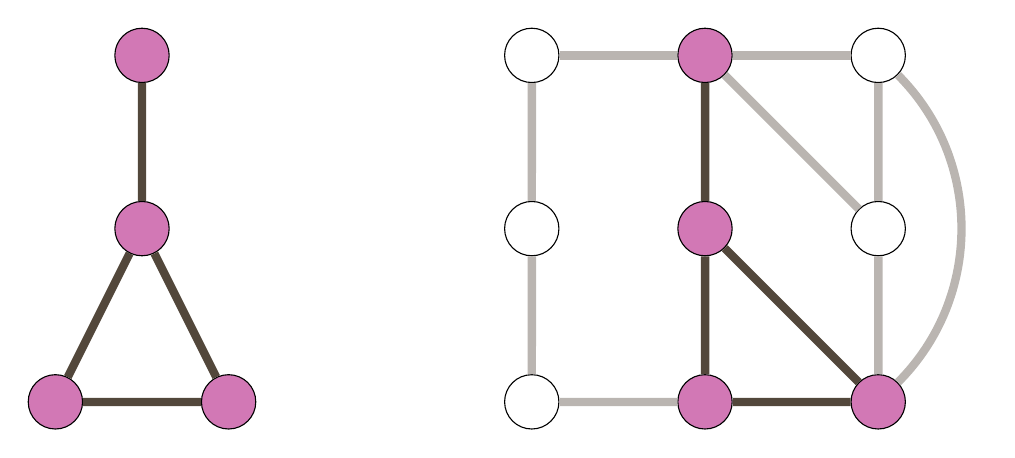
\begin{tikzpicture}[scale=1.1]%{{{
        \node[draw, circle, fill=uofgrose, inner sep=5pt, font=\bfseries] (Na) at (1,  0)
        {\vphantom{0}};
        \node[draw, circle, fill=uofgrose, inner sep=5pt, font=\bfseries] (Nb) at (1, -2)
        {\vphantom{0}};
        \node[draw, circle, fill=uofgrose, inner sep=5pt, font=\bfseries] (Nc) at (0, -4)
        {\vphantom{0}};
        \node[draw, circle, fill=uofgrose, inner sep=5pt, font=\bfseries] (Nd) at (2, -4)
        {\vphantom{0}};

        \draw [edge] (Na) -- (Nb);
        \draw [edge] (Nb) -- (Nc);
        \draw [edge] (Nc) -- (Nd);
        \draw [edge] (Nb) -- (Nd);

        \node[draw, circle, fill=uofgrose, inner sep=5pt, font=\bfseries] (N1) at (7.5,  0) {\vphantom{0}};
        \node[draw, circle, fill=white, inner sep=5pt, font=\bfseries] (N2) at (9.5,  0) {\vphantom{0}};
        \node[draw, circle, fill=uofgrose, inner sep=5pt, font=\bfseries] (N3) at (7.5, -2) {\vphantom{0}};
        \node[draw, circle, fill=white, inner sep=5pt, font=\bfseries] (N4) at (9.5, -2) {\vphantom{0}};
        \node[draw, circle, fill=uofgrose, inner sep=5pt, font=\bfseries] (N5) at (7.5, -4) {\vphantom{0}};
        \node[draw, circle, fill=uofgrose, inner sep=5pt, font=\bfseries] (N6) at (9.5, -4) {\vphantom{0}};
        \node[draw, circle, fill=white, inner sep=5pt, font=\bfseries] (N7) at (5.5,  0) {\vphantom{0}};
        \node[draw, circle, fill=white, inner sep=5pt, font=\bfseries] (N8) at (5.5, -2) {\vphantom{0}};
        \node[draw, circle, fill=white, inner sep=5pt, font=\bfseries] (N9) at (5.5, -4) {\vphantom{0}};

        \draw [ledge] (N1) -- (N2);
        \draw [edge] (N1) -- (N3);
        \draw [ledge] (N1) -- (N4);
        \draw [ledge] (N2) -- (N4);
        \draw [edge] (N3) -- (N5);
        \draw [edge] (N3) -- (N6);
        \draw [ledge] (N4) -- (N6);
        \draw [edge] (N5) -- (N6);
        \draw [ledge] (N2) to [in=45, out=315] (N6);
        \draw [ledge] (N1) -- (N7);
        \draw [ledge] (N5) -- (N9);
        \draw [ledge] (N7) -- (N8);
        \draw [ledge] (N8) -- (N9);
    \end{tikzpicture}\end{center}

    \vspace*{1.5cm}

    \begin{center}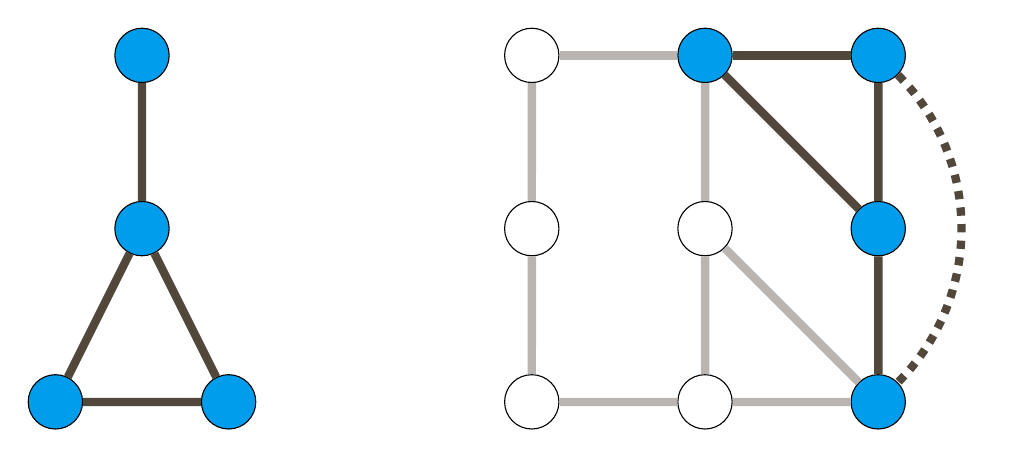
\begin{tikzpicture}[scale=1.1]%{{{
        \node[draw, circle, fill=uofgcobalt, inner sep=5pt, font=\bfseries] (Na) at (1,  0)
        {\vphantom{0}};
        \node[draw, circle, fill=uofgcobalt, inner sep=5pt, font=\bfseries] (Nb) at (1, -2)
        {\vphantom{0}};
        \node[draw, circle, fill=uofgcobalt, inner sep=5pt, font=\bfseries] (Nc) at (0, -4)
        {\vphantom{0}};
        \node[draw, circle, fill=uofgcobalt, inner sep=5pt, font=\bfseries] (Nd) at (2, -4)
        {\vphantom{0}};

        \draw [edge] (Na) -- (Nb);
        \draw [edge] (Nb) -- (Nc);
        \draw [edge] (Nc) -- (Nd);
        \draw [edge] (Nb) -- (Nd);

        \node[draw, circle, fill=uofgcobalt, inner sep=5pt, font=\bfseries] (N1) at (7.5,  0) {\vphantom{0}};
        \node[draw, circle, fill=uofgcobalt, inner sep=5pt, font=\bfseries] (N2) at (9.5,  0) {\vphantom{0}};
        \node[draw, circle, fill=white, inner sep=5pt, font=\bfseries] (N3) at (7.5, -2) {\vphantom{0}};
        \node[draw, circle, fill=uofgcobalt, inner sep=5pt, font=\bfseries] (N4) at (9.5, -2) {\vphantom{0}};
        \node[draw, circle, fill=white, inner sep=5pt, font=\bfseries] (N5) at (7.5, -4) {\vphantom{0}};
        \node[draw, circle, fill=uofgcobalt, inner sep=5pt, font=\bfseries] (N6) at (9.5, -4) {\vphantom{0}};
        \node[draw, circle, fill=white, inner sep=5pt, font=\bfseries] (N7) at (5.5,  0) {\vphantom{0}};
        \node[draw, circle, fill=white, inner sep=5pt, font=\bfseries] (N8) at (5.5, -2) {\vphantom{0}};
        \node[draw, circle, fill=white, inner sep=5pt, font=\bfseries] (N9) at (5.5, -4) {\vphantom{0}};

        \draw [edge] (N1) -- (N2);
        \draw [ledge] (N1) -- (N3);
        \draw [edge] (N1) -- (N4);
        \draw [edge] (N2) -- (N4);
        \draw [ledge] (N3) -- (N5);
        \draw [ledge] (N3) -- (N6);
        \draw [edge] (N4) -- (N6);
        \draw [ledge] (N5) -- (N6);
        \draw [hedge] (N2) to [in=45, out=315] (N6);
        \draw [ledge] (N1) -- (N7);
        \draw [ledge] (N5) -- (N9);
        \draw [ledge] (N7) -- (N8);
        \draw [ledge] (N8) -- (N9);
    \end{tikzpicture}\end{center}
\end{wrapfigure}

The \textbf{non-induced subgraph isomorphism problem} is to find an injective mapping from a given
pattern graph to a given target graph which preserves adjacency---in essence, we are ``finding a
copy of'' the pattern inside the target.

\bigskip

The \textbf{induced} variant of the problem additionally requires that the mapping preserve
non-adjacency, so there are no ``extra edges'' in the copy of the pattern that we find. The top
example is induced, whereas the bottom example is not, due to the dashed edge.

\bigskip

Despite these problems being \NP-complete, modern practical subgraph isomorphism algorithms can
handle problem instances with many hundreds of vertices in the pattern graph, and up to \textbf{ten thousand
vertices} in the target graph, leading to successful application in areas such as \textbf{computer
vision}, \textbf{biochemistry}, and \textbf{pattern recognition}. However, these algorithms cannot
handle arbitrary instances of this size---here we generate instances with thirty and one hundred and
fifty vertices respectively which cannot be solved within one hour.
}

\column{0.5}

\end{columns}

\begin{columns}
\column{0.5}

\block{See the Paper For\ldots}{
    \begin{itemize}
        \item ~ Delicious cake
    \end{itemize}
}

\column{0.5}

\block{Future Work}{
    \begin{itemize}
        \item ~ Replace Craig with James because James is better
    \end{itemize}
}

\end{columns}

{
    \colorlet{blockbodybgcolor}{uofgsandstone!80!white}
    \colorlet{blocktitlebgcolor}{uofgsandstone!80!white}
    \block[bodyverticalshift=-0.5cm]{}{
        This work was supported by the Engineering and Physical Sciences Research Council [grant
        numbers EP/K503058/1 and EP/M506539/1]. \hfill \texttt{\textcolor{white}{c.mccreesh.1@research.gla.ac.uk}}
    }
}

\end{document}

